\newpage
\subsection{Sensors}
After careful consideration, 4 water quality parameters are chosen to be monitored: turbidity, acidity, conductivity, and temperature. This set of sensors will help monitoring both the salinization issues and acidity issues at hand. Please visit the preliminary research report in Appendix A \cite{prr} for more information about these water quality parameters.

\subsubsection{Turbidity}
To measure the turbidity, the DFRobot SEN0189 \cite{SEN0189} was chosen because of it's availability and ease of hooking up.
\begin{table}[h!]
	\centering
	\adjustimage{height=4cm,valign=c}{070_design/sensors/41_sen0189.jpg}\quad
	\begin{tabular}{| l | l |}
    \hline
    Protocol & Analog\\
    Operating Temperature & 5-90 ℃ \\
    Operating Range &  0-3000NTU\\
    Response time & Within 500ms \\
    Supply Voltage & 0V-4.5V \\
    Software library included & yes \\
    Availability & 3-5 Days \\
    \hline
	\end{tabular}
\end{table}

\subsubsection{Acidity}
To measure the acidity, the DFRobot SEN0169 V2 Pro \cite{SEN0169V2} was chosen because of it's ease of hooking up and existing software libraries.
\begin{table}[h!]
	\centering
	\adjustimage{height=4cm,valign=c}{070_design/sensors/42_gravityv2pro.jpg}\quad
	\begin{tabular}{| l | l |}
    \hline
    Interface & Analog \\
    Measurement Range & 0-14 pH \\
    Measurement Accuracy &  0.1pH \\
    Response time & Within 1\gls{min} \\
    Supply Voltage & 3.3V-5V \\
    Software library included & yes \\
    Long term immersion & yes \\
    Availability & 3-5 Working Days \\
    \hline
	\end{tabular}
\end{table}

\subsubsection{Conductivity}
To measure the conductivity, the DFRobot DFR0300H \cite{DFR0300H} was chosen because of its availability and included software library.
\begin{table}[h!]
	\centering
	\adjustimage{height=4cm,valign=c}{070_design/sensors/43_dfr0300h.jpg}\quad
	\begin{tabular}{| l | l |}
    \hline
    Protocol & Analog\\
    Measurement Accuracy &  5\% \gls{FSR}\\
    Supply Voltage & 3.3-5V\\
    Support Detection Range & 10~100ms/cm\\
    Software library included & yes \\
    Probe included & yes \\
    Availability & 3-5 Working days \\
    \hline
	\end{tabular}
\end{table}

\newpage
\subsubsection{Temperature}
To measure the temperature, the DFRobot DFR0198/DS18B20 \cite{DFR0198} was chosen because of the accuracy and fast response times.
\begin{table}[h!]
	\centering
	\adjustimage{height=4cm,valign=c}{070_design/sensors/44_dfr0198.jpg}\quad
	\begin{tabular}{| l | l |}
    \hline
    Protocol & 1-Wire\\
    Measurement Range & -10-85 ℃ \\
    Measurement Accuracy &  0.5 ℃ \\
    Response time & Within 750\gls{ms} \\
    Supply Voltage & 3.3V-5V \\
    Software library included & yes \\
    Availability & 3-5 Working Days \\
    \hline
	\end{tabular}
\end{table}

\subsubsection{MCU} \label{mcu}
An Arduino Uno derivative is used as the \gls{MCU} to power and log the sensors. The board  (Vietduino \cite{vietduino}) is based on the ATmega328P microcontroller, and has a CP2102 \gls{UART}-to-Serial interface. The Vietduino has superior power delivery over the original Arduino Uno. While a more performant MCU could have been used, an Arduino was chosen because of the popular form factor and the ease of rapid prototyping. The popularity of the board makes for an excellent base for people working on this project in the future.

\begin{figure}[h]
  \centering
  \begin{minipage}[b]{0.4\textwidth}
    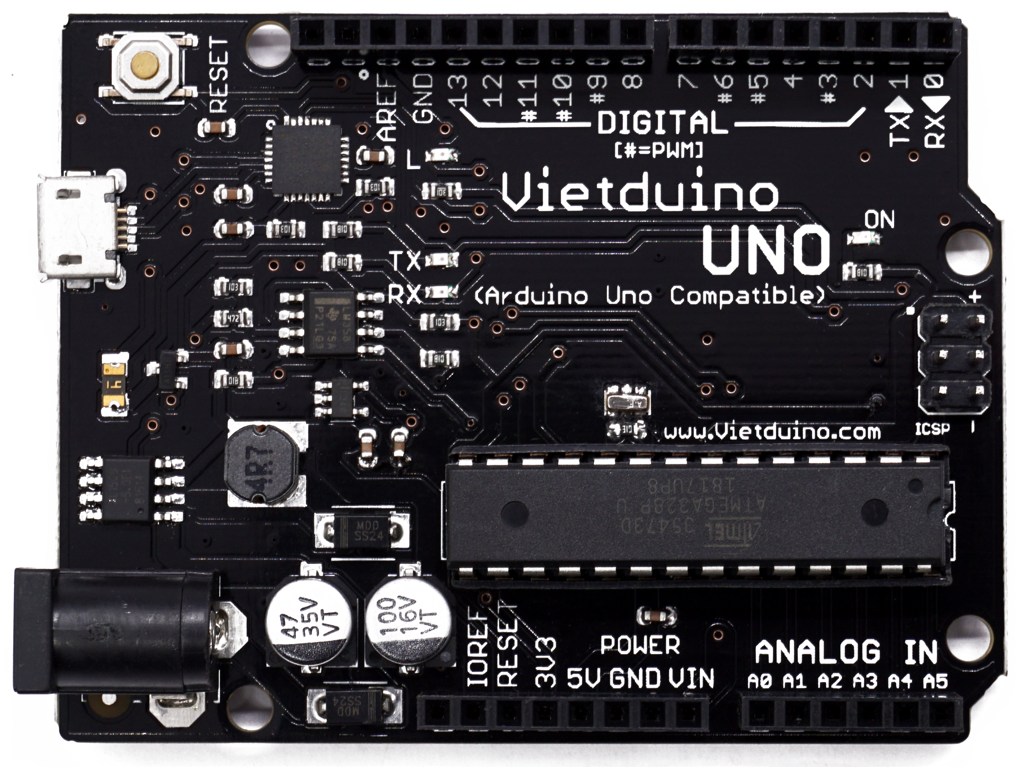
\includegraphics[width=\textwidth]{070_design/sensors/45_vietduino.png}
    \caption{Vietduino \cite{vietduino}}
  \end{minipage}
  \hfill
  \begin{minipage}[b]{0.5\textwidth}
    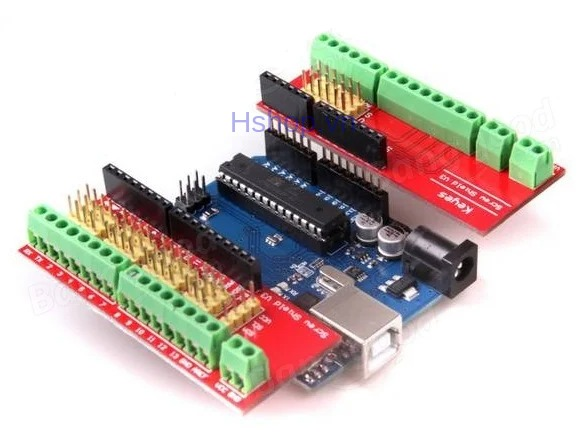
\includegraphics[width=\textwidth]{070_design/sensors/46_screwshield.jpeg}
    \caption{Screw Shield V3 \cite{screwshield}}
  \end{minipage}
\end{figure}

A screw shield was used to help with cable management and rapid prototyping. This screw shield exposes the digital and analog pins on the Arduino alongside the ground and voltage rail. This way, there is no need for any breadboard.

To log the data locally on the device, a DS3231 RTC module and SD card adapter was used.

\newpage
\subsubsection{Schematics}
In the illustration below one can find the schematics of the sensors and the microcontroller board.
\begin{figure}[h]
\centering
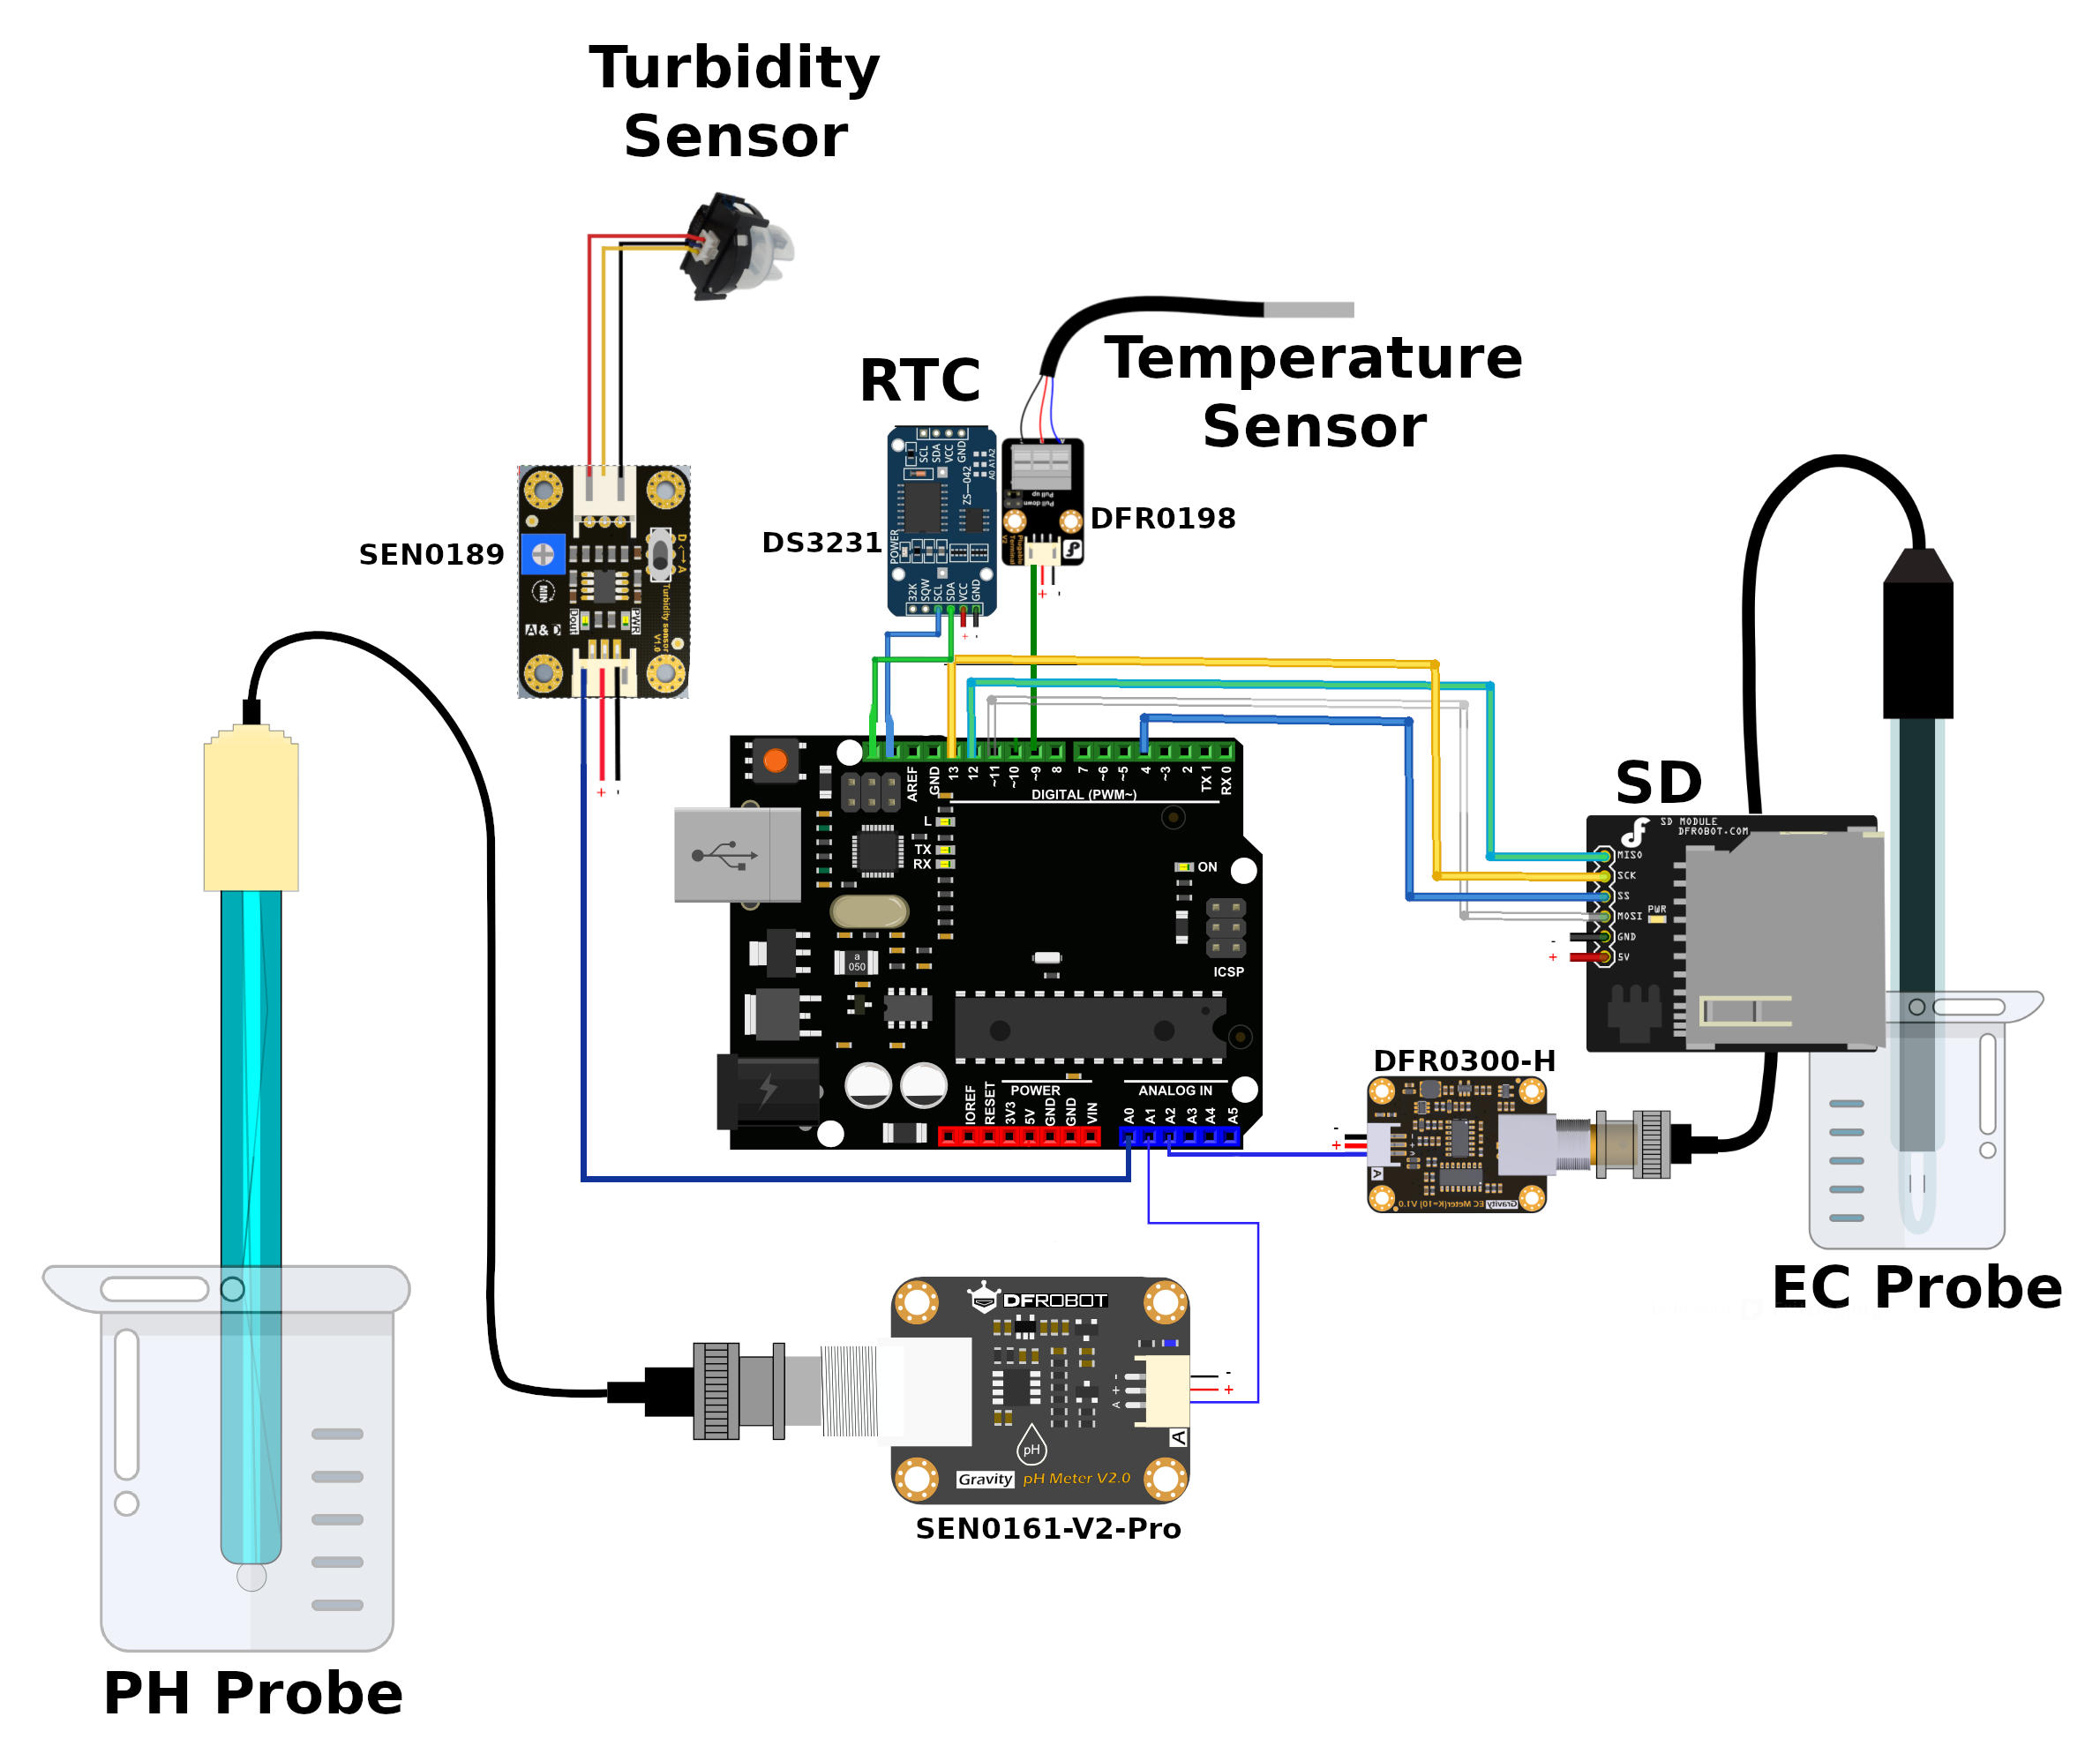
\includegraphics[scale=0.8]{070_design/sensors/47_schematic.png}
\caption{MCU and sensors schematic [own picture]}
\end{figure}

